\documentclass[10pt, final]{article}

\usepackage{cite}
\usepackage{fullpage}
\usepackage{graphicx}
\usepackage{hyperref}
\usepackage{amsmath}
\usepackage{subcaption}
\usepackage{url}
\usepackage[ruled,vlined,commentsnumbered,titlenotnumbered, norelsize]{algorithm2e}

% Line break with additional spacing. Default is .75 line-height extra spacing
% Extra space is put in to allow line breaks immediately after \item
\newcommand{\br}[1][.75]{\ \\[#1\baselineskip]}

\parindent 0pt

\begin{document}

\begin{center}
\LARGE{\textbf{Training a Pok\'{e}mon Puzzle League Champion}}\\
\Large{\textbf{CS 221 Project Progress Report}}\\
\Large{Logan Short, Christopher Wong}
\end{center}

\section{Introduction}
Pok\'{e}mon Puzzle League is a puzzle game released by Nintendo in September 2000 for the Nintendo 64 entertainment system. The goal of our project is to develop an AI agent that can play the game at a high level. In this progress report, we expand upon the ideas introduced in our proposal by (1) giving motivation for our AI strategy by explaining game mechanics, (2) providing our final implementation techniques for extracting and modeling board game state, and (3) detailing our algorithms to calculate the best move for any given board state. We conclude with the next steps we plan to take to finish up our project.

\section{General Game Strategy}
For general gameplay instructions, see Section $2$ of our proposal. We add on that, in the $2$-player ``Versus'' mode, clearing many blocks quickly causes garbage blocks to be sent to the opponent's board. To destroy garbage blocks, one can make a $3$-in-a-row (or larger) adjacent to a garbage block. This will deconstruct the garbage block into random normal blocks, thus allowing them to be cleared normally.\br
In either mode, the player gets extra benefit by creating combos and chains. Combos are created when there are more than $3$ blocks cleared at one time. A chain is created when, after a clear, blocks fall to create additional clears. Figure~\ref{fig:chain} demonstrates a simple chain taking place. Chains are more valuable than combos.
\begin{figure}[h!]
\centerline{
\begin{subfigure}[h]{1.3in}
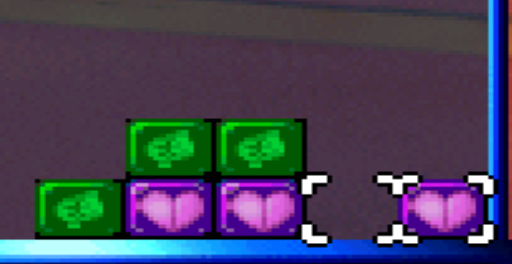
\includegraphics[width=1.3in]{chain1.png}
\end{subfigure}
~$\mathbf{\Longrightarrow}$~
\begin{subfigure}[h]{1.3in}
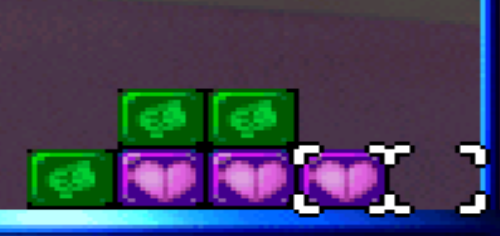
\includegraphics[width=1.3in]{chain2.png}
\end{subfigure}
~$\mathbf{\Longrightarrow}$~
\begin{subfigure}[h]{1.3in}
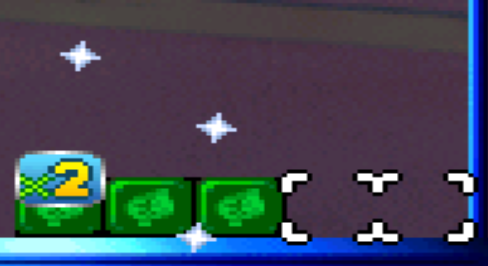
\includegraphics[width=1.3in]{chain3.png}
\end{subfigure}}
\caption{Clearing a simple $2$x chain.}
\label{fig:chain}
\end{figure}

\subsection{Differences between Modes}
In each mode, the player wants to create large combos and long chains, while preventing his or her grid from reaching the top. Doing so will either score more points or hurt the opponent with larger garbage blocks. With this in mind, we think that optimal game strategy is largely the same in both modes. So, for our progress report, we have focused only on a single AI that can be used for either mode. The one difference between modes is the priority to clear garbage blocks, which we will discuss as a next step in Section $6$.

\section{Game State Model}
Since we do not have access to the internal data of the game, we can rely only on what is being displayed on screen. So, we first built an interface that allows us to capture in-game screenshots and send movements to the game multiple times per second. Our end-to-end system will thus loop the following steps quickly: (1) Capture an in-game screenshot, (2) Check if the game has ended, (3) Extract the board state from the screenshot, (4) Calculate the best move(s) possible on the board, and (5) Send the move(s) to the game.

\subsection{Board Recognition}
Given a screenshot, we extract and classify the grid squares from the agent's board. To do so, we used OpenCV to isolate and divide the board. We then used a logistic regression classifier to determine the type of each block. It turns out that the best feature vector for each block image was simply taking the RGB values of each pixel, since all grid blocks of the same type always look identical. Rising blocks introduces the problem that the bottom grid is not always flush with the bottom of the game screen. To solve this, we consider the block-sized image at each possible vertical position of the lower left block. Using our classifier, we calculate the likelihood that each image is an actual block, and we pick the position that yields the highest probability. The final challenge rested in being able to differentiate the background from an actual block. As a workaround, we always chose the same game settings so that the background does not vary. Then, we divided the background itself into a grid and trained on it as well. Thus, our classifier was now able to guess the \texttt{BACKGROUND} class, which we would subsequently treat as an empty grid cell.

% \subsection{Internal Representation}
% Since we can accurately classify all of the blocks on the board, it is straightforward for us to represent an internal board state as a grid that is $6$ wide and $12$ tall. There are a finite number of block types (along with garbage and empty), so we can enumerate all possible values that a grid cell can take. Our internal model also accounts for gravity and is able to calculate future boards resulting from potential switches.

\section{Algorithm}
Given the game mechanics, there are several considerations that must be accounted for when deciding on an optimal algorithm:
(1) Since the game is played in real time, our algorithm for calculating an optimal set of moves must be able to return a strong set of moves relatively quickly. Consequently, an algorithm that is able to produce decent moves in a short amount of time is preferable to an algorithm that returns very strong moves but requires a large amount of processing time.
(2) The board state only changes when a swap is made. Moving the cursor around the board does not affect the position of pieces in any way. Our algorithms can thus focus on the optimal swaps, while leaving the necessary cursor movements to get there as a secondary concern.
(3) High level gameplay revolves around setting up combos and chains that can be set off by one swap. As such, it is better to attempt to find an optimal sequence of ``setup'' swaps that leads to one very influential swap, instead of trying to find optimal singleton swaps one at a time. \br
Given these considerations, we decided to explore the space of randomized algorithms that evaluate sequences of moves using a defined evaluation function. The strength of the algorithms in this space lies in their ability to quickly determine sequences of moves that yield relatively strong results. This fits our needs well since it is not necessary that we perform an exhaustive search to find a board's true optimal sequence of moves.
\subsection{Board Evaluation}
The primary goal for our board evaluation function is to give high scores to boards that contain large combos and chains and give lower scores to boards that do not result in very many pieces being cleared. In addition, since chains yield better results than combos and longer chains are the best, our evaluation function should favor long chains over large combos. We thus decided to go with a simple evaluation function that mapped this relationship directly. If we define $B$ to be a board, $S(B)$ to be the score of $B$, and $k_i$ to be the number of pieces matched and cleared at chain multiplier $i$ for the board $B$, our evaluation function is of the form:
\begin{align*}
S(B) = \sum_{i}i \cdot k_i
\end{align*}
\subsection{Random Algorithm}
Our first approach is a Random Algorithm that works by generating a series of sequences of random board position swaps. Each sequence is then applied to the board and the board evaluation scores after each swap are summed to obtain the final score of the move sequence. The sequence which yields the highest score is returned as the chosen move sequence. The variables for this algorithm are the number of randomly generated sequences to test and the number of swaps used in a sequence. Increasing the number of tested sequences tends to yield better results at the cost of runtime. Increasing the number of moves in a sequence tends to yield larger combos and chains but also increases the runtime.
\begin{algorithm}\label{random}\small
\caption{\small Random Algorithm$(B, numTrials, numMoves)$}
$\alpha \gets 0$ \\
$\beta \gets $ empty list\\
\ForEach{$i \in $ range(0,numTrials)}{
$\alpha' \gets 0$ \\
$\beta' \gets$ generate random sequence of $numMoves$ swaps \\
\ForEach{$m \in \beta'$}{
$B \gets$ Apply $m$ to $B$ \\
$\alpha' \gets \alpha' + Evaluate(B)$
}
rollback $B$ \\
\If{$s > \alpha$}{
$\alpha \gets \alpha'$ \\
$\beta \gets \beta'$ \\
}
}
return $\alpha, \beta$
\end{algorithm}
\subsection{Genetic Algorithm}
Building upon the Random Algorithm, we decided to implement a Genetic Algorithm which attempts to combine the best parts of randomly generated move sequences in order to produce a more optimal sequence. Our Genetic Algorithm which begins by generating a set of random swap sequences, $S$. Each of these move sequences is then scored by summing the evaluation scores of the resulting board after each swap in the sequence. A new generation of sequences is then formed by selecting two sequences from $S$. During this selection process, the probability of selecting a sequence $a$ is based on the relative score of $a$ in comparison to all other sequences in $S$, with higher scores yielding higher probabilities. Once two sequences have been selected, a pivot index is picked uniformly at random. A child is generated by concatenating all the swaps up to the pivot index of one sequence with all the swaps after the pivot point of the other sequence. Thus this process generates two children. These children are added to a new sequence set $S'$ and the child generating process is continued until the size of $S'$ is equal to the size of $S$. We then set $S$ to be equal to $S'$ and repeat the process. After a specified number of generations, we return the move sequence in $S$ that yields the highest score. \br
Variables for this algorithm include the size of the set $S$, the number of generations to run, and the length of a move sequence. As with the Random Algorithm, increasing these parameters yields better results at the cost of increased runtime. An additional variable is the probability distribution of sequence selection based on the scores. Initial testing seems to indicate that having the selection probability be based on a distribution made up of the squares of sequence scores yields favorable results.
\begin{algorithm}\label{genetic}\small
\caption{\small Genetic Algorithm$(B, numSeq, numGen, numMoves)$}
$S \gets$ list of $numSeq$ random sequences of $numMoves$ swaps\\
\ForEach{$i \in$ range(0,numGen)}{
$S' \gets$ empty list\\
$seq1 \gets$ pick from $S$ with probability based on Evaluate() score \\
$seq2 \gets$ pick from $S$ with probability based on Evaluate() score \\
$p \gets$ uniformly random value in $range(0,numMoves)$ \\
$child1 \gets seq1[0:p] + seq2[p:numMoves]$ \\
$child2 \gets seq2[0:p] + seq1[p:numMoves]$ \\
append $child1, child2$ to $S'$ \\
$S \gets S'$
}
return sequence in $S$ with best Evaluate() score\\
\end{algorithm}

\section{Results}
Before moving forward with the implementation of mapping keyboard inputs to perform the move sequences returned by our algorithms, we decided to focus on the tuning of our algorithm variables to yield a desirable balance between move optimality and processing time. Evaluation was performed by running out algorithms on randomly generated board states. The primary factors we focused on were move sequence and runtime.\br
A description of our baseline and oracle are given in Section $4.3$ of our proposal. This section also gives baseline and oracle results for ``Versus'' mode. We add on that, in ``Endless'' mode, our baseline got an average score of $2460$, and our oracle got an average score of $18781$.

\section{Next Steps}
We are pleased with our progress on our project so far. Our end-to-end system will have a lot of moving parts that must execute in quick cycles. We have already done much of the work and analysis to optimize the core code that calculates the best move. Finishing our robust interface for game communication is not a concern. As for our AI algorithm, there are still other ideas we would like to try to improve our results. In particular, we plan to account for:
\begin{itemize}
\item Incorporating column height into our evaluation. A player loses the game even if one pesky column -- clearly higher than the rest -- reaches the top. Our AI may sometimes have to make switches which ``topple'' the column, even if the switch does not directly lead to any combos or chains.
\item Supporting advanced timing techniques for dynamic chains. Gravity is not instantaneous after blocks are cleared. Many new chains are possible if a player can sneak key blocks beneath other falling blocks. This will need a fine-tuned game interface, with accuracy to the tenth of a second.
\item Utilizing the existence of garbage blocks to improve our AI in ``Versus'' modes. Right now, we have one AI which works reasonably well in both modes. However, as mentioned earlier, in ``Versus'' mode, clearing garbage blocks is a priority. This means that we can optimize our $2$-player AI by accounting for garbage blocks. A stretch goal would be to analyze the opponent's board as well, to see what possible garbage blocks may be incoming.
\end{itemize}

\newpage

\section{Appendix}
Below is an example sequence produced by our genetic algorithm. As can be seen, it is capable of detecting complex setups that lead to large combos and long chains. To help locate block switches, we give the left coordinate of the cursor as (row, col), $0$-indexed, with $(0,0)$ as the bottom-left. The first four moves are quick block switches for setup.
\begin{figure}[ht!]
\centerline{
\begin{subfigure}[h]{1.3in}
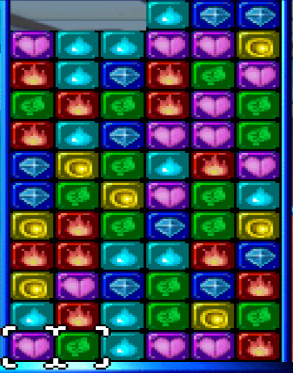
\includegraphics[width=1.3in]{inspirational1.png}
\caption*{Start: $(0,0)$}
\end{subfigure}
~$\mathbf{\Longrightarrow}$~
\begin{subfigure}[h]{1.3in}
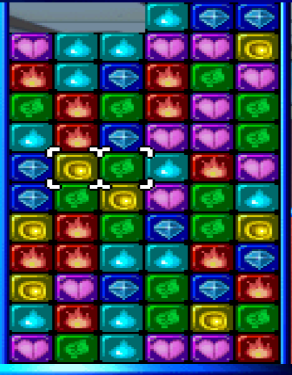
\includegraphics[width=1.3in]{inspirational2.png}
\caption*{Red-blue: $(7,0)$}
\end{subfigure}
~$\mathbf{\Longrightarrow}$~
\begin{subfigure}[h]{1.3in}
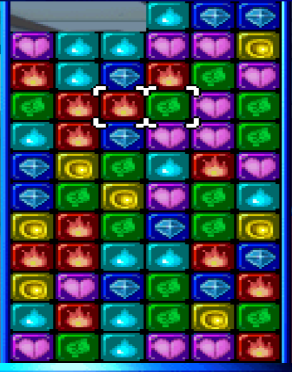
\includegraphics[width=1.3in]{inspirational3.png}
\caption*{Green-red: $(8,2)$}
\end{subfigure}
~$\mathbf{\Longrightarrow}$~
\begin{subfigure}[h]{1.3in}
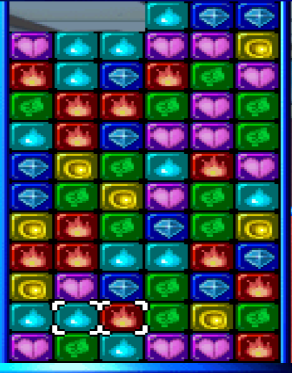
\includegraphics[width=1.3in]{inspirational4.png}
\caption*{Red-blue: $(1,1)$}
\end{subfigure}}\end{figure}

\vspace{-.1in}
\begin{figure}[h!]
We continue to set up our chain. Four more block switches that clear some blocks in between. Note that our model must account for board state changes during the sequence.\br
\centerline{
\begin{subfigure}[h]{1.3in}
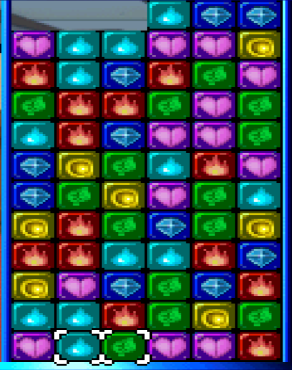
\includegraphics[width=1.3in]{inspirational5.png}
\caption*{Green-blue: $(0,1)$}
\end{subfigure}
~$\mathbf{\Longrightarrow}$~
\begin{subfigure}[h]{1.3in}
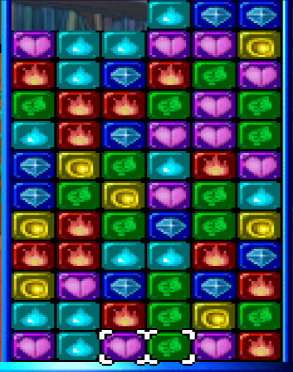
\includegraphics[width=1.3in]{inspirational6.png}
\caption*{Green-pink: $(0,2)$ \\ Three in a row!}
\end{subfigure}
~$\mathbf{\Longrightarrow}$~
\begin{subfigure}[h]{1.3in}
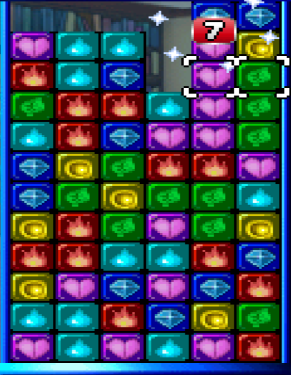
\includegraphics[width=1.3in]{inspirational7.png}
\caption*{Green-pink: $(9,4)$ \\ $7$-combo!}
\end{subfigure}
~$\mathbf{\Longrightarrow}$~
\begin{subfigure}[h]{1.3in}
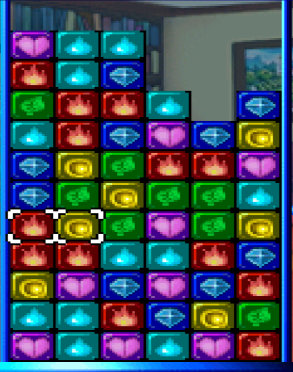
\includegraphics[width=1.3in]{inspirational8.png}
\caption*{Red-yellow: $(4,0)$}
\end{subfigure}}\end{figure}

\vspace{-.1in}
\begin{figure}[h!]
One last switch to start a great chain! About half of the blocks have been cleared after $8$ switches.\br
\centerline{
\begin{subfigure}[h]{1.3in}
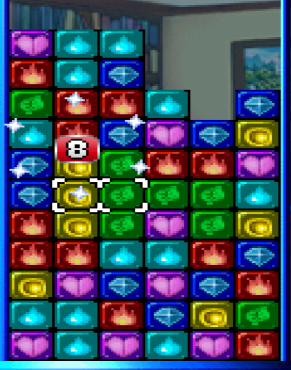
\includegraphics[width=1.3in]{inspirational9.png}
\caption*{Green-yellow: $(5,1)$ \\ $8$-combo!}
\end{subfigure}
~$\mathbf{\Longrightarrow}$~
\begin{subfigure}[h]{1.3in}
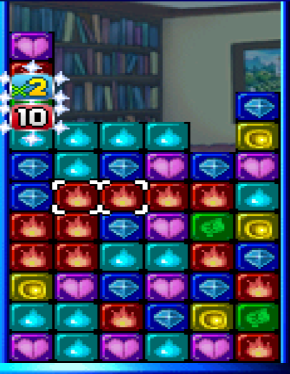
\includegraphics[width=1.3in]{inspirational10.png}
\caption*{$2$x chain + $10$-combo!}
\end{subfigure}
~$\mathbf{\Longrightarrow}$~
\begin{subfigure}[h]{1.3in}
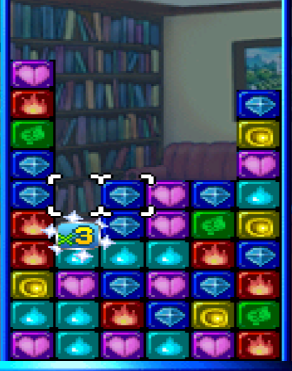
\includegraphics[width=1.3in]{inspirational11.png}
\caption*{$3$x chain!}
\end{subfigure}
~$\mathbf{\Longrightarrow}$~
\begin{subfigure}[h]{1.3in}
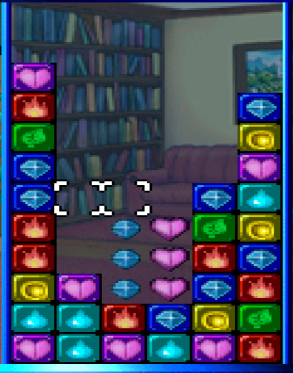
\includegraphics[width=1.3in]{inspirational12.png}
\caption*{$4$x chain + $6$-combo!}
\end{subfigure}}\end{figure}

% \begin{figure}[h!]\begin{center}
% 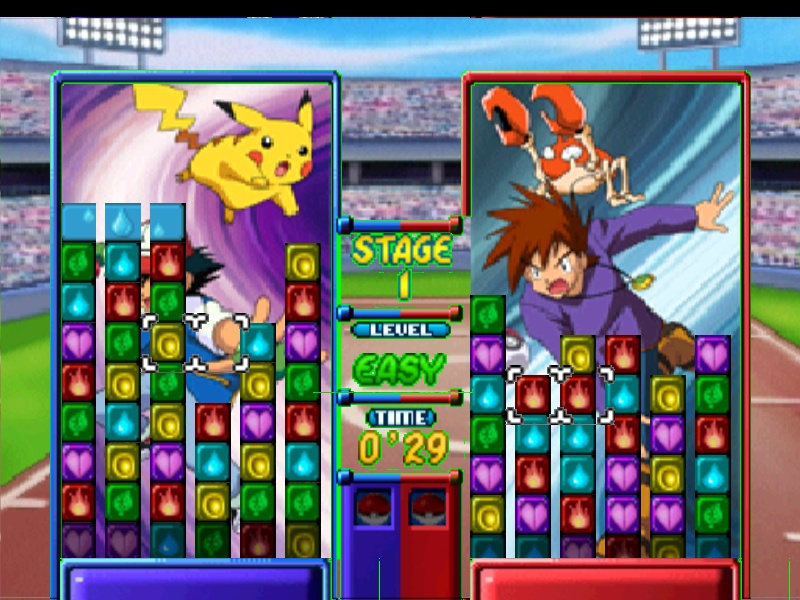
\includegraphics[width=3.4in]{game.jpg}
% \caption{Example game screen in $2$-player mode. The human player or agent is on the left.}
% \label{fig:screenshot}
% \end{center}\end{figure}
% \begin{figure}[h!]\begin{center}
% \begin{subfigure}[h]{1.6in}
% 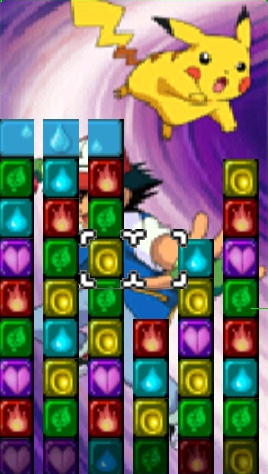
\includegraphics[width=1.6in]{board.jpg}
% \caption*{Isolate the agent's board.}
% \end{subfigure}
% ~$\mathbf{\Longrightarrow}$~
% \begin{subfigure}[h]{1.6in}
% 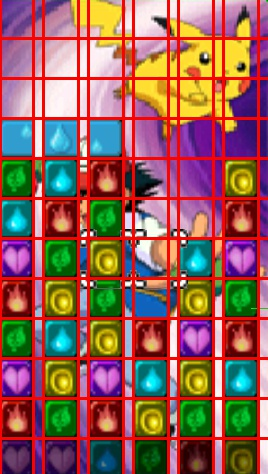
\includegraphics[width=1.6in]{grid.jpg}
% \caption*{Divide board into a grid.}
% \end{subfigure}
% ~$\mathbf{\Longrightarrow}$~
% \begin{subfigure}[h]{1.2in}
%   \begin{subfigure}[h]{.5in}
%   
\includegraphics[]{square0.jpg}
%   \caption*{$(0,0)$}
%   \end{subfigure}
%   ~
%   \begin{subfigure}[h]{.5in}
%   
\includegraphics[]{square1.jpg}
%   \caption*{$(0,1)$}
%   \end{subfigure}
%   \caption*{Extract squares.}
% \end{subfigure}
% \caption{Process of parsing the grid game state from the game screen.}
% \label{fig:extract}
% \end{center}\end{figure}

\end{document}